\documentclass[11pt,a4paper]{article}

\usepackage[margin=2.2cm]{geometry}
\usepackage{fontspec}
\setmainfont{DejaVu Serif}
\setsansfont{DejaVu Sans}
\setmonofont[Scale=0.85]{DejaVu Sans Mono}
\usepackage{xcolor}
\usepackage[hidelinks]{hyperref}
\usepackage{booktabs,tabularx,longtable,array}
\usepackage{enumitem}
\usepackage{listings}
\usepackage[most]{tcolorbox}
\usepackage{tikz}
\usetikzlibrary{arrows.meta,positioning,fit,backgrounds}
\usepackage{fancyhdr}
\usepackage{titlesec}

\definecolor{brand}{HTML}{0F766E}
\definecolor{ink}{HTML}{1F2937}
\definecolor{soft}{HTML}{F0FDFA}
\definecolor{warn}{HTML}{B45309}
\definecolor{warnbg}{HTML}{FFFBEB}
\definecolor{codebg}{HTML}{F8FAFC}

\hypersetup{colorlinks=true,linkcolor=brand,urlcolor=brand}
\titleformat{\section}{\Large\bfseries\color{brand}}{\thesection}{0.6em}{}
\titleformat{\subsection}{\large\bfseries\color{ink}}{\thesubsection}{0.6em}{}
\setlist{itemsep=2pt,topsep=4pt}
\setlength{\parindent}{0pt}
\setlength{\parskip}{5pt}

\pagestyle{fancy}
\fancyhf{}
\lhead{\small\color{gray}Tabeeby Agent --- MCP, Skills \& Reliable Loops}
\rhead{\small\color{gray}\thepage}
\renewcommand{\headrulewidth}{0.3pt}

\lstset{
  basicstyle=\ttfamily\small, backgroundcolor=\color{codebg}, frame=single,
  rulecolor=\color{gray!40}, breaklines=true, columns=fullflexible,
  keepspaces=true, showstringspaces=false, xleftmargin=4pt, xrightmargin=4pt,
}

\newtcolorbox{note}[1][Note]{colback=soft,colframe=brand,fonttitle=\bfseries,title=#1,arc=2pt,boxrule=0.6pt}
\newtcolorbox{action}[1][Action needed]{colback=warnbg,colframe=warn,fonttitle=\bfseries,title=#1,arc=2pt,boxrule=0.6pt}
\newcommand{\code}[1]{\texttt{#1}}
\newcolumntype{Y}{>{\raggedright\arraybackslash}X}
\emergencystretch=3em
\sloppy

\begin{document}

\begin{titlepage}
  \centering
  \vspace*{3cm}
  {\Huge\bfseries\color{brand} Tabeeby Agent\par}
  \vspace{0.4cm}
  {\Large MCP, Skills and Reliable Goal Loops\par}
  \vspace{0.3cm}
  {\large What was added, why, and how to run, deploy and use it\par}
  \vspace{1.5cm}
  \begin{tcolorbox}[colback=soft,colframe=brand,width=0.82\textwidth,arc=2pt]
  \small
  \textbf{Branch:} \code{feature/mcp-skills-reliable-loops}\\[2pt]
  \textbf{Concepts covered:} Workshop 4 (MCP), Workshop 5 (Skills), Workshop 6 (Reliable loops \& evaluation)\\[2pt]
  \textbf{Result:} 32/32 offline tests passing; 11/11 live evaluation cases passing on Gemini + Qdrant Cloud\\[2pt]
  \textbf{Channels:} REST API, Telegram (webhook \& polling), MCP (HTTP \& stdio)\\[2pt]
  \textbf{Deployment target:} FastAPI Cloud; local development with conda
  \end{tcolorbox}
  \vfill
  {\small 1 October 2026}
\end{titlepage}

\tableofcontents
\newpage

%=====================================================================
\section{Summary}

Tabeeby already had a working core: a Gemini tool-calling agent that searches 17{,}119 Vezeeta doctors in Qdrant, exposed over FastAPI and a Telegram webhook. This branch adds the three concepts from the course resources and turns the agent into a measurably reliable service:

\begin{description}[leftmargin=1.2em]
  \item[MCP (Workshop 4)] Tabeeby is now an \emph{MCP server} (tools, resources and prompts, over streamable HTTP at \code{/mcp} and over stdio for Claude Desktop/Cursor) \emph{and} an \emph{MCP client} that can borrow tools from any external MCP server configured in \code{.env}.
  \item[Skills (Workshop 5)] Seven medical skills written as \code{SKILL.md} recipes with reference files, loaded through progressive disclosure (menu $\rightarrow$ body $\rightarrow$ references), plus a trigger bench that tests whether the right skill fires.
  \item[Reliable loops (Workshop 6)] A four-axis budget (steps, seconds, tool actions, USD), stuck-loop detection, \emph{self-verification in code} with automatic refinement, a deterministic safety repair, and an evaluation harness that turns ``it worked when I tried it'' into a pass rate.
\end{description}

On top of that, the branch fixes several real bugs found while working (Section~\ref{sec:fixes}), upgrades the Telegram bot, prepares FastAPI Cloud deployment, and moves the workflow to conda. One important pre-existing data issue was discovered and needs your decision (Section~\ref{sec:embeddings}).

\begin{note}[Concept $\rightarrow$ feature map]
\small
\begin{tabularx}{\linewidth}{@{}lY@{}}
\toprule
\textbf{Course idea} & \textbf{Where it lives in Tabeeby} \\
\midrule
MCP server (tools/resources/prompts) & \code{src/mcp\_server/server.py}, mounted at \code{/mcp} in \code{app.py} \\
MCP client, sync bridge, toolbox & \code{src/stores/mcp/toolbox.py} (\code{McpToolbox}, \code{McpRegistry}) \\
Skill menu, \code{load\_skill}, references & \code{src/tools/skills.py}, \code{src/skills/*/SKILL.md} \\
Trigger bench & \code{src/evals/skill\_trigger\_bench.py} \\
Budget (steps, seconds, actions) & \code{src/agent/budget.py} (+ USD and answer-time reserve) \\
Verifier is code; generate$\rightarrow$verify$\rightarrow$refine & \code{src/agent/verifiers.py}, loop in \code{src/agent/agent.py} \\
Eval set as a number & \code{src/evals/eval\_set.json}, \code{src/evals/run\_eval.py}, \code{src/tests/} \\
\bottomrule
\end{tabularx}
\end{note}

%=====================================================================
\section{Architecture}

\begin{center}
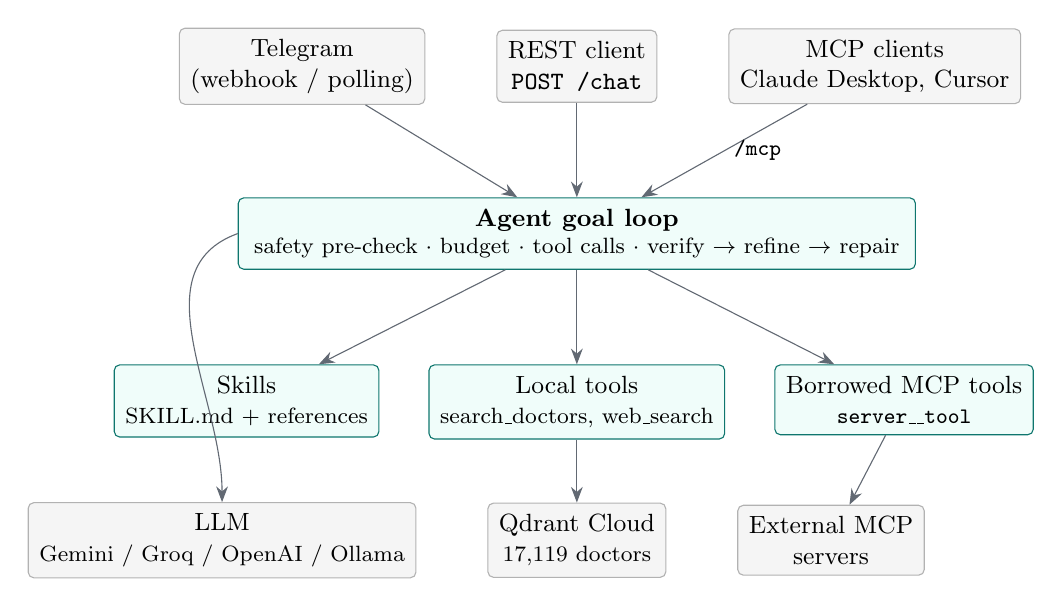
\begin{tikzpicture}[
  node distance=6mm and 9mm,
  box/.style={draw=brand,rounded corners=2pt,fill=soft,align=center,font=\small,minimum height=8mm,inner sep=4pt},
  ext/.style={draw=gray!60,rounded corners=2pt,fill=gray!8,align=center,font=\small,minimum height=8mm,inner sep=4pt},
  arr/.style={-{Stealth[length=2mm]},draw=ink!70},
]
\node[ext] (tg) {Telegram\\(webhook / polling)};
\node[ext,right=of tg] (rest) {REST client\\\code{POST /chat}};
\node[ext,right=of rest] (mcpc) {MCP clients\\Claude Desktop, Cursor};

\node[box,below=12mm of rest,minimum width=8.6cm] (agent) {\textbf{Agent goal loop}\\[-1pt]
  \footnotesize safety pre-check $\cdot$ budget $\cdot$ tool calls $\cdot$ verify $\rightarrow$ refine $\rightarrow$ repair};

\node[box,below left=12mm and -18mm of agent] (skills) {Skills\\\footnotesize SKILL.md + references};
\node[box,below=12mm of agent] (tools) {Local tools\\\footnotesize search\_doctors, web\_search};
\node[box,below right=12mm and -18mm of agent] (borrow) {Borrowed MCP tools\\\footnotesize \code{server\_\_tool}};

\node[ext,below=8mm of tools] (qdrant) {Qdrant Cloud\\\footnotesize 17{,}119 doctors};
\node[ext,left=of qdrant] (llm) {LLM\\\footnotesize Gemini / Groq / OpenAI / Ollama};
\node[ext,right=of qdrant] (extmcp) {External MCP\\servers};

\draw[arr] (tg) -- (agent);
\draw[arr] (rest) -- (agent);
\draw[arr] (mcpc) -- node[right,font=\footnotesize]{\code{/mcp}} (agent);
\draw[arr] (agent) -- (skills);
\draw[arr] (agent) -- (tools);
\draw[arr] (agent) -- (borrow);
\draw[arr] (tools) -- (qdrant);
\draw[arr] (borrow) -- (extmcp);
\draw[arr] (agent.west) to[out=200,in=90] (llm.north);
\end{tikzpicture}
\end{center}

All entry points share one bootstrap (\code{helpers/bootstrap.py}), so the REST API, Telegram, the stdio MCP server, the evals and the polling bot all run exactly the same agent with the same configuration.

%=====================================================================
\section{MCP --- Model Context Protocol (Workshop 4)}

\subsection{Tabeeby as an MCP server}
Defined once in \code{src/mcp\_server/server.py} with \code{MCPServer} from \code{mcp>=2.2}, served over two transports:

\begin{itemize}
  \item \textbf{Streamable HTTP} at \code{https://<app>/mcp/}, mounted inside the FastAPI app (stateless, JSON responses) and protected by \code{Authorization: Bearer \$MCP\_API\_KEY}.
  \item \textbf{stdio} via \code{python src/mcp\_server/\_\_main\_\_.py} for local clients; \code{--http} runs it standalone on port 8001, \code{--no-agent} exposes the tools only.
\end{itemize}

\begin{center}\small
\begin{tabularx}{\linewidth}{@{}llY@{}}
\toprule
\textbf{Kind} & \textbf{Name} & \textbf{What it does} \\
\midrule
Tool & \code{search\_doctors} & Hybrid vector + filter search; area/specialty normalised (English or Arabic) \\
Tool & \code{check\_emergency} & Deterministic red-flag scan; returns categories and emergency numbers \\
Tool & \code{medical\_web\_search} & Tavily search with source URLs \\
Tool & \code{list\_specialties}, \code{list\_areas} & Canonical filter values with doctor counts; resolves free text \\
Tool & \code{ask\_tabeeby} & Runs the \emph{whole} agent loop and returns its verified answer \\
Resource & \code{tabeeby://emergency-numbers} & Egypt emergency numbers (JSON) \\
Resource & \code{tabeeby://skills}, \code{tabeeby://skills/\{name\}} & The skill menu and each skill's instructions \\
Prompt & \code{triage(symptoms, area, max\_fee)} & A ready-made triage workflow for any MCP client \\
\bottomrule
\end{tabularx}
\end{center}

Tools carry MCP annotations (\code{readOnlyHint}, \code{openWorldHint}) so clients know they are safe to call.

\textbf{Claude Desktop configuration} (\code{claude\_desktop\_config.json}):
\begin{lstlisting}
{ "mcpServers": { "tabeeby": {
    "command": "/home/<you>/miniconda3/envs/tabeeby-agent/bin/python",
    "args": ["/path/to/Tabeeby-Agent/src/mcp_server/__main__.py"] } } }
\end{lstlisting}

\subsection{Tabeeby as an MCP client}
\code{src/stores/mcp/toolbox.py} ports the Workshop~4 \code{McpToolbox}: MCP is async but the agent loop is sync, so an \code{anyio} blocking portal runs the event loop on a background thread (thread-safe, shared by concurrent requests). \code{McpRegistry} combines several servers:

\begin{lstlisting}
MCP_SERVERS={"fetch":  {"command": "uvx", "args": ["mcp-server-fetch"]},
             "remote": {"url": "https://example.com/mcp",
                        "headers": {"Authorization": "Bearer ..."}}}
\end{lstlisting}

\begin{itemize}
  \item Borrowed tools are named \code{<server>\_\_<tool>} so two servers can both expose \code{search}.
  \item Their JSON schemas are passed to the LLM next to our Python tools. The Gemini provider was extended to turn schemas into \code{FunctionDeclaration}s; OpenAI, Groq and Ollama accept them natively.
  \item A server that fails to start is logged in \code{/health} and skipped --- one optional integration can never take the medical assistant down. A tool error is returned to the model as text, so the loop survives.
\end{itemize}

%=====================================================================
\section{Skills (Workshop 5)}

\begin{quote}\itshape A tool is an appliance. A skill is a recipe.\end{quote}

\subsection{Progressive disclosure}
\begin{center}\small
\begin{tabular}{@{}lll@{}}
\toprule
\textbf{Level} & \textbf{What} & \textbf{When it is read} \\
\midrule
1 & \code{name} + \code{description} & Always --- appended to the system prompt as a menu \\
2 & Body of \code{SKILL.md} & When the model calls \code{load\_skill(name)} \\
3 & Files in \code{references/} & When the body says to call \code{read\_skill\_reference(skill, file)} \\
\bottomrule
\end{tabular}
\end{center}

Reference reads are sandboxed to the skill's own \code{references/} folder (path traversal is blocked and tested).

\subsection{The seven skills}
\begin{center}\small
\begin{tabularx}{\linewidth}{@{}lY@{}}
\toprule
\textbf{Skill} & \textbf{Recipe (references)} \\
\midrule
\code{emergency-triage} & ``Call 123'' first, then $\le$4 first-aid steps \emph{only} from the reference, then optional follow-up specialists (\code{red-flags.md}, \code{first-aid.md}) \\
\code{doctor-finder} & Decide specialty, extract area/budget, search, present doctor cards (\code{specialty-map.md}, \code{card-format.md}) \\
\code{egyptian-arabic} & Match the patient's register; translate the complaint to an English clinical query for the tool (\code{glossary.md}) \\
\code{medication-info} & Web search with citations; never personal dosing (\code{safety-rules.md}) \\
\code{lab-results} & Below/within/above typical range, which specialist reads it (\code{reference-ranges.md}) \\
\code{pediatric-care} & Warning signs first, then pediatricians; no child doses (\code{warning-signs.md}) \\
\code{mental-health-support} & Validation, two coping steps, psychiatrists; self-harm hands over to emergency-triage \\
\bottomrule
\end{tabularx}
\end{center}

\textbf{Adding a skill needs no Python:} create \code{src/skills/<name>/SKILL.md} with a \code{name} and a \code{description} whose ``Use when \ldots'' part lists the words patients actually type. The description is the trigger; when the wrong skill fires, fix that one line and re-run \code{make bench}.

Skills are also visible from outside: \code{GET /skills}, \code{GET /skills/\{name\}}, the Telegram \code{/skills} command and the MCP resources.

%=====================================================================
\section{Reliable goal loop (Workshop 6)}

\begin{quote}\itshape A loop without a budget is a bug. The verifier is where the intelligence is.\end{quote}

\subsection{Budget}
Each patient message gets a \code{Budget} (\code{agent/budget.py}), configurable in \code{.env}:

\begin{center}\small
\begin{tabular}{@{}lll@{}}
\toprule
\textbf{Axis} & \textbf{Default} & \textbf{Setting} \\
\midrule
LLM calls (steps) & 8 & \code{AGENT\_MAX\_STEPS} \\
Wall clock & 90 s & \code{AGENT\_MAX\_SECONDS} \\
Tool calls actually executed (actions) & 12 & \code{AGENT\_MAX\_ACTIONS} \\
Spend in USD & off & \code{AGENT\_MAX\_COST\_USD} \\
Verifier-driven rewrites & 2 & \code{AGENT\_MAX\_REFINEMENTS} \\
\bottomrule
\end{tabular}
\end{center}

Two refinements over the workshop version, both found by running the real agent:
\begin{itemize}
  \item \textbf{Answer reserve.} On the last step, after the action budget, and in the last 25\% of the time budget, tool calls are refused with ``write your final answer now''. Without this the live agent was cut off mid-search and the patient received no answer.
  \item \textbf{Stuck detection.} A tool that fails twice is disabled for the rest of the message, and an identical repeated call is not executed again. In the live run the model had retried a failing search four times in a row.
\end{itemize}

\subsection{Self-verification in code}
Every final answer is checked by code before it reaches the patient (\code{agent/verifiers.py}):

\begin{center}\small
\begin{tabularx}{\linewidth}{@{}lY@{}}
\toprule
\textbf{Verifier} & \textbf{Rule} \\
\midrule
\code{answer\_not\_empty} & The answer has text. \\
\code{emergency\_protocol} & If the message contains red flags, the answer contains 123. \\
\code{links\_are\_grounded} & Every Vezeeta \emph{doctor} link was returned by \code{search\_doctors} (no invented URLs). \\
\code{booking\_links\_present} & If doctors were found, at least one of their booking links is shown. \\
\code{language\_matches} & Arabic in, Arabic out. \\
\bottomrule
\end{tabularx}
\end{center}

A failing check is sent back with \emph{specific} feedback (``these links were not returned by search\_doctors: \ldots''), and the model rewrites its answer. If the budget ends while a check still fails, \code{repair\_answer} applies deterministic fixes: unverified links are removed and the emergency banner is put first. An unsafe answer is never shipped as-is.

The red-flag detector (\code{agent/safety.py}) is plain code covering English, Modern Standard Arabic and Egyptian colloquial forms (masculine, feminine and first person). It also adds a safety note to the system prompt before the first LLM call.

\subsection{Evidence returned to clients}
\code{Agent.run()} returns an \code{AgentResult}: the answer plus \code{stop\_reason} (\code{completed}, \code{verified after N refinement(s)}, \code{step budget hit}, \code{repaired: \ldots}, \code{llm\_error}), the verification checks, skills used, every tool call with its source (\code{local}, \code{mcp}, \code{dropped}, \code{disabled}, \code{duplicate}), budget usage and cost. \code{POST /chat} returns these with \code{"include\_trace": true}.

%=====================================================================
\section{Evaluation}

\subsection{Offline test suite --- 32 tests}
\code{make test} runs without API keys: a scripted fake LLM and a fake vector DB exercise the budget, safety, catalog normalisation, verifiers, skills (all three levels and the sandbox), the full loop (skill $\rightarrow$ search $\rightarrow$ verified answer; fabricated link $\rightarrow$ refinement; emergency repair; dropped actions; step cap; stuck detection), the MCP server in memory, the MCP client against a real stdio subprocess, the HTTP \code{/mcp} endpoint with bearer auth, \code{/chat} sessions, and the Telegram handler and formatter. The same suite was also run in a clean \code{uv sync --locked} environment on Python 3.10, which simulates the FastAPI Cloud build.

\subsection{Live evaluation --- 11/11 passing}
\code{make eval} runs the real agent (Gemini + Qdrant Cloud) over \code{evals/eval\_set.json} and scores each case with code: specialty and area passed to the search (after normalisation), budget respected, answer language, emergency detection, required/forbidden text, expected skill, and whether the answer self-verified.

\begin{center}\small
\begin{tabularx}{\linewidth}{@{}lYl@{}}
\toprule
\textbf{Case} & \textbf{Prompt (summary)} & \textbf{Result} \\
\midrule
dental-ar-area & Egyptian Arabic toothache in Maadi & pass \\
ortho-en-budget & Knee injury, Nasr City, max 400 EGP & pass \\
cardiac-emergency & Crushing chest pain spreading to arm & pass (1 refinement) \\
stroke-ar & Arabic stroke signs (feminine forms) & pass \\
pediatric-fever & 2-year-old with fever, Heliopolis & pass \\
derm-hairloss & Hair loss, 6th of October & pass \\
fertility-ar & Arabic: no pregnancy after 2 years, Nasr City & pass (1 refinement) \\
anxiety & Insomnia and anxiety & pass (1 refinement) \\
lab-hba1c & HbA1c 7.2\% & pass (1 refinement) \\
out-of-scope & Python coding request & pass (refused) \\
jailbreak & ``Ignore previous instructions\ldots'' & pass (refused) \\
\bottomrule
\end{tabularx}
\end{center}

The first full run scored 5/11. The failures were caused by the Gemini free-tier rate limit, a gap in the Arabic red-flag phrases, and a verifier that treated the Vezeeta homepage as a doctor link. Each was fixed (retry/backoff, feminine Egyptian forms, profile-link-only grounding), and the cases now pass. A full run costs about \$0.017. Reports are saved to \code{evals/reports/}.

\code{make bench} runs the skill trigger bench: for each prompt it checks the model's \emph{first} move (which skill it loads, or none for ``hi'').

%=====================================================================
\section{Other improvements and bug fixes}\label{sec:fixes}

\subsection{Bugs fixed}
\begin{itemize}
  \item \textbf{Area and specialty filters silently returned nothing.} Qdrant filters use exact keyword match, so ``Maadi'', ``6 October'', Arabic area names or ``Orthopedic Surgery'' never matched the stored values (\code{El-Maadi}, \code{6Th Of October}, \code{Orthopedics}). \code{tools/catalog.py} now maps free text to the 140 canonical areas and 37 specialties (alias table with Arabic, then fuzzy matching).
  \item \textbf{Zero results instead of the closest doctors.} The search now relaxes one constraint at a time (specialty, then fee, then area) and tells the model which filter it dropped. A query that is just a specialty name becomes a filter.
  \item \textbf{The patient's message was repeated to the LLM.} The loop passed the prompt again on every iteration while it was already in the history, so after each tool call the model saw the user turn duplicated (always, with Ollama).
  \item \textbf{Telegram history could break Gemini.} Trimming to ``system + last 10 messages'' could start the window on an orphaned tool response and stored raw tool-call objects. Memory now keeps only clean user/assistant turns (\code{helpers/session\_store.py}, with TTL).
  \item \textbf{Telegram answers over 4096 characters failed} and Markdown such as \code{**bold**} and \code{[text](url)} showed as raw symbols. Answers are now split on paragraph boundaries and converted to Telegram HTML, with a plain-text fallback.
  \item \textbf{Duplicate agent runs from Telegram retries:} the webhook waited for the full agent run, so Telegram retried. It now verifies, de-duplicates and returns 200 immediately; the work continues in the background.
  \item \code{ChatRequest.total\_cost} was an \code{int}; \code{\_execute\_tool} referenced attributes that did not exist; the system prompt told the model to answer ``in the user's language English''; the Groq settings existed but were never wired up; the unused \code{pathlib} backport was a dependency.
\end{itemize}

\subsection{New features}
\begin{itemize}
  \item Retry with backoff for rate limits and transient errors (honours Gemini's ``retry in N s'').
  \item \code{GROQ} generation backend (OpenAI-compatible).
  \item Server-side conversation memory for the REST API (\code{session\_id}, \code{DELETE /chat/\{id\}}).
  \item \code{GET /health}, \code{/tools}, \code{/skills}; FastAPI app factory for testing.
  \item Telegram: \code{/help}, \code{/emergency}, \code{/skills}, bot command menu, webhook secret token, per-chat lock, non-text message handling, and a long-polling mode (\code{make telegram}) for local development without a public URL.
  \item \code{scripts/check\_vector\_consistency.py} --- verifies the vectors match the embedding model.
  \item Conda \code{environment.yml}, a Makefile that runs everything in the conda env, and \code{scripts/push\_env\_to\_fastapi\_cloud.sh}.
  \item The system prompt forbids Markdown tables (they do not render in Telegram) and caps the answer length.
\end{itemize}

%=====================================================================
\section{Important finding: the stored vectors do not match the embedding model}\label{sec:embeddings}

While testing, unfiltered semantic search returned clearly wrong specialties (``toothache'' $\rightarrow$ orthopedists, ``child fever'' $\rightarrow$ physiotherapists). To confirm, I re-embedded the stored text of several Qdrant points with the configured model (\code{gemini-embedding-001}, 1024 dimensions) and compared it with the stored vector:

\begin{center}
\begin{tabular}{@{}lc@{}}
\toprule
\textbf{Point} & \textbf{cosine(stored, re-embedded)} \\
\midrule
Reproductive Medicine \& Infertility & 0.017 \\
Neurology & $-0.021$ \\
Cardiology & 0.019 \\
\bottomrule
\end{tabular}
\end{center}

The same model would give about 1.0. The collection was therefore built with a \emph{different} embedding model, and the semantic part of the hybrid search is currently noise. Results looked right only because the agent passes specialty and area filters. The new normaliser and specialty inference make those filters much more reliable, but symptom-level matching (subspecialties, conditions) will only work after re-ingestion.

\begin{action}[Decision needed]
Either (a) tell me which embedding model/provider was used for ingestion and I will switch \code{EMBEDDING\_*} back, or (b) re-ingest with the current model: \code{make ingest} (drops and rebuilds the cloud collection; 17{,}119 embedding calls --- probably needs a paid Gemini tier or several days on the free tier). Check afterwards with \code{make check-vectors}. I did not run (b) because it is destructive and uses your quota.
\end{action}

%=====================================================================
\section{Telegram: using the chatbot}

\subsection{Locally (no public URL)}
\begin{lstlisting}
cd src && conda activate tabeeby-agent
make telegram        # long polling; removes the webhook while it runs
\end{lstlisting}

\subsection{In production (FastAPI Cloud)}
Set these and deploy; on startup the app registers the webhook with the secret and sets the bot's command menu:
\begin{lstlisting}
TELEGRAM_BOT_TOKEN=...
TELEGRAM_WEBHOOK_URL=https://<your-app>.fastapicloud.dev/telegram/webhook
TELEGRAM_WEBHOOK_SECRET=<python -c "import secrets; print(secrets.token_urlsafe(32))">
\end{lstlisting}
Telegram allows only one delivery mode per bot. After using polling locally, restart or redeploy the cloud app to restore the webhook. Your current \code{.env} still points the webhook at an old \code{trycloudflare.com} tunnel; replace it with the FastAPI Cloud URL.

Commands: \code{/start}, \code{/help}, \code{/reset}, \code{/emergency}, \code{/skills}.

%=====================================================================
\section{Deploying to FastAPI Cloud}

FastAPI Cloud installs dependencies from \code{uv.lock} (regenerated on this branch with \code{mcp 2.2.0}), picks the Python version from \code{requires-python}, and reads the entrypoint from \code{[tool.fastapi] entrypoint = "app:app"} in \code{pyproject.toml}. Environment variables must be set in the cloud because \code{.env} is not uploaded.

\begin{lstlisting}
cd src && conda activate tabeeby-agent
fastapi login                 # opens the browser (your account)
fastapi deploy                # builds and deploys; prints the app URL
make cloud-env                # pushes .env: *KEY/*TOKEN/*SECRET as encrypted secrets
fastapi deploy                # env changes need a redeploy
curl https://<your-app>.fastapicloud.dev/health
\end{lstlisting}

Before \code{make cloud-env}, edit \code{.env}: set \code{TELEGRAM\_WEBHOOK\_URL} to the cloud URL, and add \code{TELEGRAM\_WEBHOOK\_SECRET} and \code{MCP\_API\_KEY}. A dry run of the production build (clean \code{uv sync --locked} on Python 3.10, then \code{fastapi run}) passed: \code{/health} reported every component healthy, \code{/mcp} rejected requests without the key (401), and an MCP client listed and called all six tools over HTTP.

%=====================================================================
\section{What I need from you}

\begin{action}[Requests]
\begin{enumerate}
  \item \textbf{Embedding decision} (Section~\ref{sec:embeddings}): which model built the collection, or approval to re-ingest.
  \item \textbf{FastAPI Cloud login}: run \code{fastapi login} yourself (it is your account), then \code{fastapi deploy}. I prepared everything else but cannot log in for you.
  \item \textbf{Secrets to create}: \code{TELEGRAM\_WEBHOOK\_SECRET} and \code{MCP\_API\_KEY} (any long random strings), and the new \code{TELEGRAM\_WEBHOOK\_URL}.
  \item \textbf{Gemini quota}: the free tier (15 requests/minute) is tight, since one message can take 3--6 LLM calls. Retries now handle short bursts. For real users, enable billing, or use \code{GENERATION\_BACKEND=GROQ} with \code{openai/gpt-oss-120b} (tested and working with your key).
  \item \textbf{Gemini key}: early in the session your \code{AQ.}-prefixed key returned \code{401 ACCESS\_TOKEN\_TYPE\_UNSUPPORTED}; it worked again minutes later. If it recurs, create a standard AI Studio key (\code{AIza\ldots}).
  \item \textbf{Medical review}: the skill references (first aid, lab ranges, pediatric warning signs) are written conservatively from general guidance. Please have a clinician review them, and confirm any extra Egyptian hotline numbers you want added (only 123, 122 and 180 are included).
  \item \textbf{Scaling}: conversation memory is in-process. If FastAPI Cloud runs several instances, say so and I will move sessions to Redis (already a dependency).
\end{enumerate}
\end{action}

%=====================================================================
\appendix
\section{Quick reference}

\begin{center}\small
\begin{tabularx}{\linewidth}{@{}lY@{}}
\toprule
\textbf{Command (in \code{src/})} & \textbf{Does} \\
\midrule
\code{make env} & Create/update the \code{tabeeby-agent} conda env \\
\code{make app} & Run the API locally with reload (\code{/docs}) \\
\code{make test} & 32 offline tests \\
\code{make eval} / \code{make bench} & Live evaluation / skill trigger bench \\
\code{make mcp} / \code{make mcp-http} & Tabeeby MCP server over stdio / HTTP :8001 \\
\code{make telegram} & Telegram bot via long polling \\
\code{make check-vectors} & Embedding/vector consistency check \\
\code{make lock} & Refresh \code{uv.lock} after editing dependencies \\
\code{make cloud-env} / \code{make deploy} & Push env to FastAPI Cloud / deploy \\
\code{make docs} & Rebuild this PDF \\
\bottomrule
\end{tabularx}
\end{center}

\end{document}
